\documentclass[12pt,compress,ngerman,utf8,t]{beamer}
\usepackage{etex}
\usepackage[ngerman]{babel}
\usepackage{ragged2e}
\usepackage{tabto}
\usepackage{wasysym}
\usepackage{booktabs}
\usepackage{mathtools}
\usepackage{tikz}
\usetikzlibrary{calc}
\usepackage[all]{xy}
\usepackage[protrusion=true,expansion=false]{microtype}

\DeclareSymbolFont{extraup}{U}{zavm}{m}{n}
\DeclareMathSymbol{\varheart}{\mathalpha}{extraup}{86}
\DeclareMathSymbol{\vardiamond}{\mathalpha}{extraup}{87}

\DeclareUnicodeCharacter{2237}{$\dblcolon$}
\DeclareUnicodeCharacter{21D2}{$\Rightarrow$}
\DeclareUnicodeCharacter{2192}{$\rightarrow$}

\title[Was sind und was sollen die Typen?]{\smiley{} Was sind und was sollen die Typen? \smiley}
\author[Augsburger Curry Club]{\textcolor{white}{Ingo Blechschmidt \\ Curry Club Augsburg}}
\date[2016-07-14]{\textcolor{white}{14. April 2016}}

\usetheme{Warsaw}

\useinnertheme{rectangles}

\usecolortheme{seahorse}
\definecolor{mypurple}{RGB}{150,0,255}
\setbeamercolor{structure}{fg=mypurple}
\definecolor{myred}{RGB}{150,0,0}
\setbeamercolor*{title}{bg=myred,fg=white}
\setbeamercolor*{titlelike}{bg=myred,fg=white}

\usefonttheme{serif}
\usepackage[T1]{fontenc}
\usepackage{libertine}

\newcommand{\slogan}[1]{%
  \begin{center}%
    \setlength{\fboxrule}{2pt}%
    \setlength{\fboxsep}{8pt}%
    {\usebeamercolor[fg]{item}\fbox{\usebeamercolor[fg]{normal text}\parbox{0.33\textwidth}{#1}}}%
  \end{center}%
}

\definecolor{darkred}{RGB}{220,0,0}
\newcommand{\hcancel}[5]{%
    \tikz[baseline=(tocancel.base)]{
        \node[inner sep=0pt,outer sep=0pt] (tocancel) {#1};
        \draw[darkred, line width=1mm] ($(tocancel.south west)+(#2,#3)$) -- ($(tocancel.north east)+(#4,#5)$);
    }%
}%

\renewcommand{\C}{\mathcal{C}}
\newcommand{\D}{\mathcal{D}}
\newcommand{\id}{\mathrm{id}}
\newcommand{\Id}{\mathrm{Id}}
\newcommand{\Hask}{\mathrm{Hask}}
\newcommand{\defeq}{\vcentcolon=}
\newcommand{\base}{\mathsf{base}}
\newcommand{\lloop}{\mathsf{loop}}
\newcommand{\surf}{\mathsf{surf}}
\newcommand{\merid}{\mathsf{merid}}
\renewcommand{\U}{\mathcal{U}}
\newcommand{\ap}{\mathsf{ap}}
\newcommand{\IsEquiv}{\mathsf{IsEquiv}}
\newcommand{\fib}{\mathsf{fib}}
\newcommand{\UIP}{\mathsf{UIP}}
\newcommand{\ZZ}{\mathbb{Z}}
\newcommand{\inv}{\mathsf{inv}}
\newcommand{\defeqv}{\vcentcolon\equiv}
\newcommand{\IsContr}{\mathsf{IsContr}}
\newcommand{\refl}{\mathsf{refl}}
\newcommand{\IsMereProp}{\mathsf{IsMereProp}}
\newcommand{\NN}{\mathbb{N}}
\newcommand{\ct}{%
  \mathchoice{\mathbin{\raisebox{0.5ex}{$\displaystyle\centerdot$}}}%
             {\mathbin{\raisebox{0.5ex}{$\centerdot$}}}%
             {\mathbin{\raisebox{0.25ex}{$\scriptstyle\,\centerdot\,$}}}%
             {\mathbin{\raisebox{0.1ex}{$\scriptscriptstyle\,\centerdot\,$}}}
}

\setbeamertemplate{navigation symbols}{}
\setbeamertemplate{headline}{}

\setbeamertemplate{title page}[default][colsep=-1bp,rounded=false,shadow=false]
\setbeamertemplate{frametitle}[default][colsep=-2bp,rounded=false,shadow=false,center]

\newcommand*\oldmacro{}%
\let\oldmacro\insertshorttitle%
\renewcommand*\insertshorttitle{%
  \oldmacro\hfill\insertframenumber\,/\,\inserttotalframenumber\hfill}

\newcommand{\hil}[1]{{\usebeamercolor[fg]{item}{\textbf{#1}}}}
\setbeamertemplate{frametitle}{%
  \vskip1em%
  \leavevmode%
  \begin{beamercolorbox}[dp=1ex,center]{}%
      \usebeamercolor[fg]{item}{\textbf{\textsf{\Large \insertframetitle}}}
  \end{beamercolorbox}%
}

\setbeamertemplate{footline}{%
  \leavevmode%
  \hfill%
  \begin{beamercolorbox}[ht=2.25ex,dp=1ex,right]{}%
    \usebeamerfont{date in head/foot}
    \insertframenumber\,/\,\inserttotalframenumber\hspace*{1ex}
  \end{beamercolorbox}%
  \vskip0pt%
}

\newcommand{\backupstart}{
  \newcounter{framenumberpreappendix}
  \setcounter{framenumberpreappendix}{\value{framenumber}}
}
\newcommand{\backupend}{
  \addtocounter{framenumberpreappendix}{-\value{framenumber}}
  \addtocounter{framenumber}{\value{framenumberpreappendix}}
}

\setbeameroption{show notes}
\setbeamertemplate{note page}[plain]

\newcommand{\imgslide}[1]{{\usebackgroundtemplate{\parbox[c][\paperheight][c]{\paperwidth}{\centering\includegraphics[height=\paperheight]{#1}}}\begin{frame}[plain]\end{frame}}}
\newcommand{\imgslideW}[1]{{\usebackgroundtemplate{\parbox[c][\paperheight][c]{\paperwidth}{\centering\includegraphics[width=\paperwidth]{#1}}}\begin{frame}[plain]\end{frame}}}

\begin{document}

% http://www.unoosa.org/res/timeline/index_html/space-2.jpg
{\usebackgroundtemplate{
\includegraphics[height=\paperheight]{images/space}}
\frame{\titlepage}}

{\usebackgroundtemplate{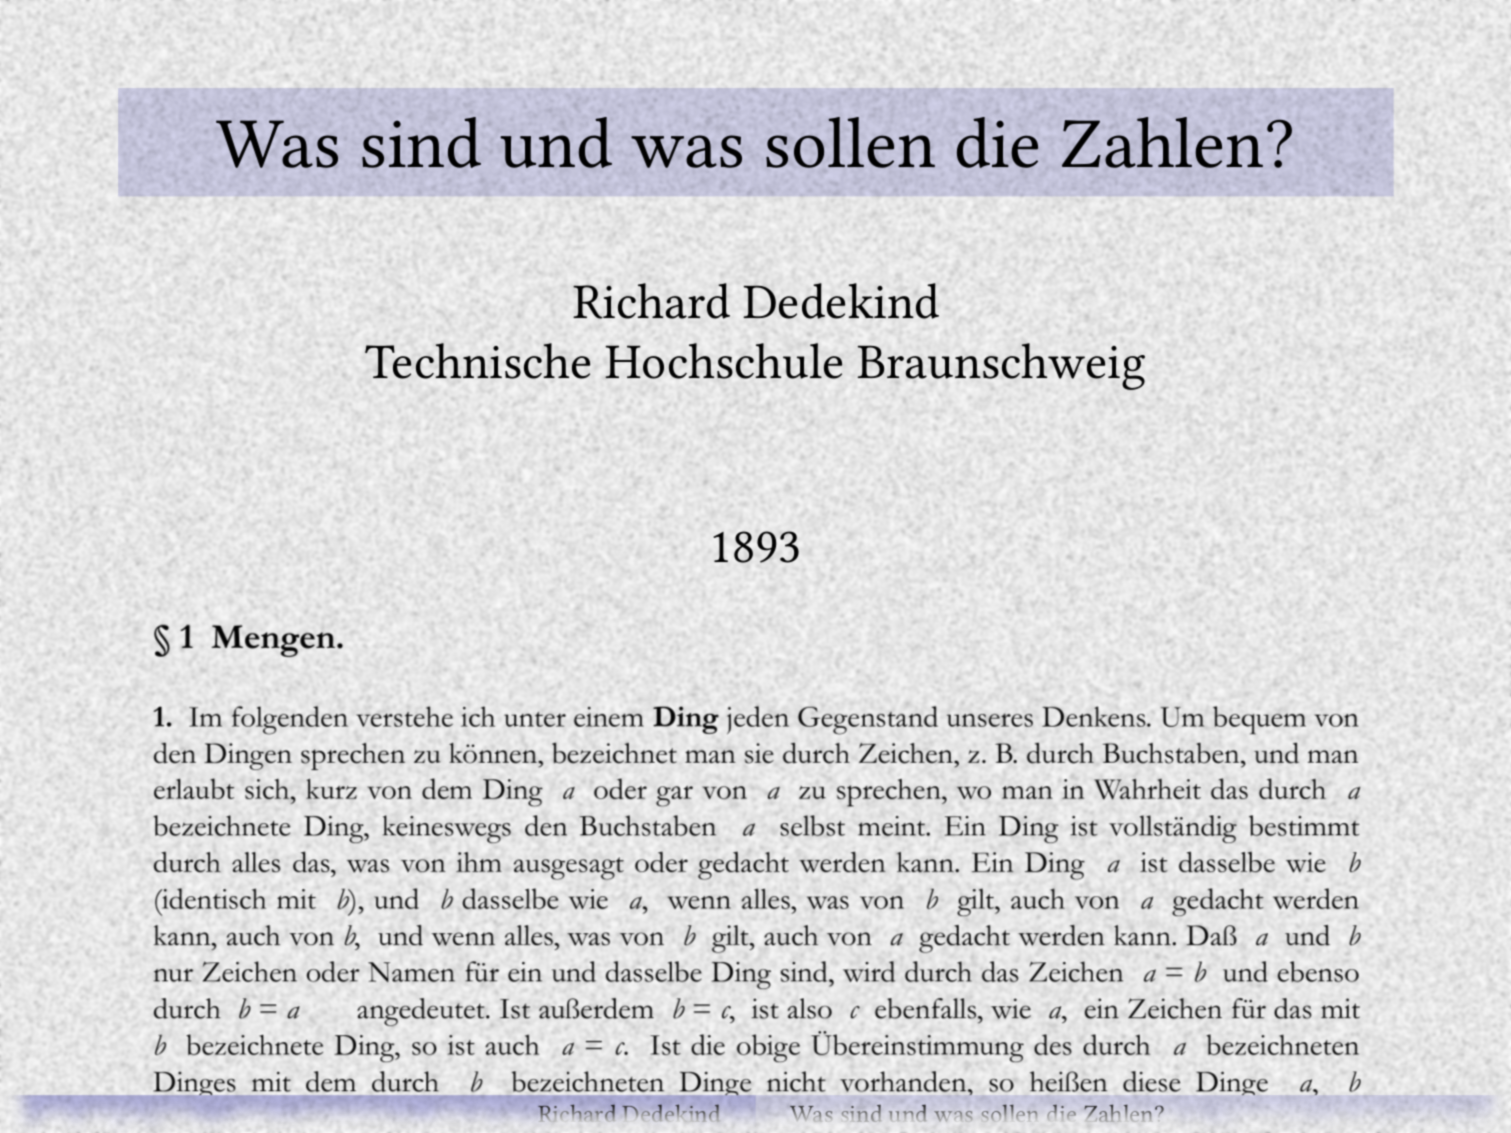
\includegraphics[height=\paperheight]{images/dedekind-titleslide}}
\frame{}}

\frame{\tableofcontents}


\section{Vorgeschichte}

\begin{frame}{Was sind Grundlagen?}
  \begin{itemize}
    \item Grundlagen liefern den logischen Rahmen für Mathe.
    \item Ihre Details spielen oft keine Rolle.
    \item Aber ihre wesentlichen Konzepte schon.
  \end{itemize}

  \bigskip
  \centering
  
\includegraphics[scale=0.25]{images/bridge}
  \par
\end{frame}

\imgslideW{images/logicomix-1}
\imgslideW{images/logicomix-2}


\note{
  \begin{itemize}
    \item\justifying Grundlagen erlauben uns, maximal präzise zu sein.
    \item Ein \emph{Beweis} im üblichen mathematischen Sinn ist eine Anleitung,
    wie ein (niemals ausbuchstabierter) vollständig formaler Beweis zu
    konstruieren wäre.
    \item Die Korrektheit von formalen Beweisversuchen kann -- anders als bei
    informalen Beweisversuchen -- maschinell geprüft werden.
  \end{itemize}
}

\note{
  \begin{itemize}
    \item\justifying Es gibt kein Theorem der Art "`Das Sonnensystem ist genau
    dann stabil, wenn das folgende Axiom über große Kardinalzahlen gilt"'.
    Resultate in der Mathematik hängen nur sehr selten von speziellen Details
    der Fundierung ab.

    \item Brücken werden nicht zusammenbrechen, wenn eine Logikerin eine
    Inkonsistenz in Zermelo--Fraenkel-Mengenlehre findet.
  \end{itemize}
}

\begin{frame}[plain,c]
  \begin{columns}[c]
    \begin{column}{0.6\textwidth}
      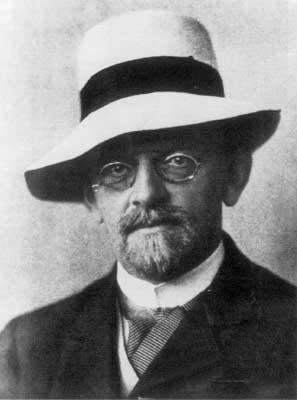
\includegraphics[scale=0.8]{images/hilbert}
    \end{column}
    \begin{column}{0.4\textwidth}
      Aus dem Paradies, das Cantor uns geschaffen, soll uns niemand vertreiben
      können.\medskip

      -- David Hilbert, 1926

      \bigskip
      \bigskip
      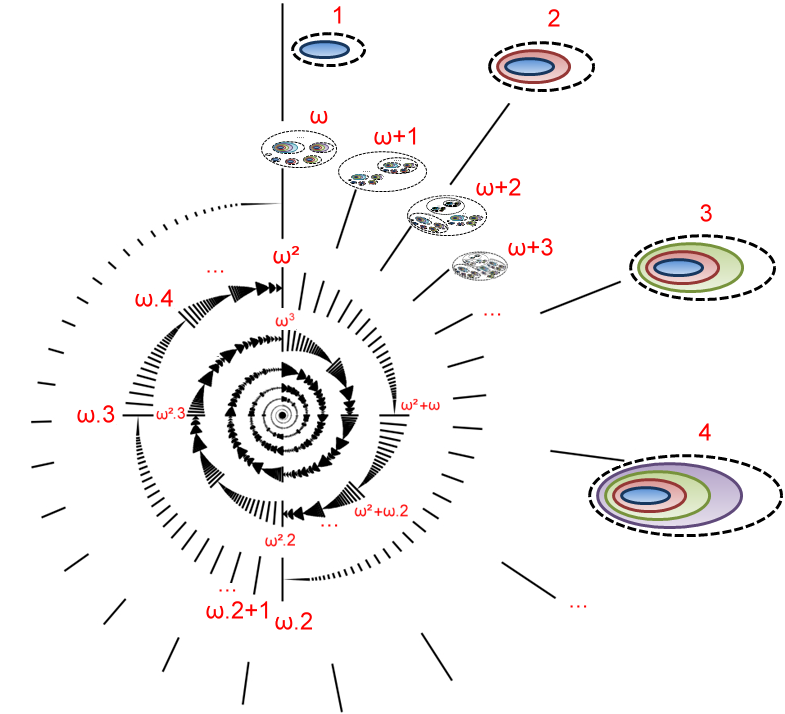
\includegraphics[width=\textwidth]{images/ordinal-numbers}
    \end{column}
  \end{columns}
\end{frame}

\imgslide{images/principia-mathematica}
\imgslide{images/principia-mathematica-1plus1}

{\logo{
\includegraphics[scale=0.3]{images/paradox}}
\begin{frame}{Paradoxa}
  \begin{itemize}
    \item Paradox von Richard
    \item Paradox von Curry
    \item Die Russellsche Antinomie
  \end{itemize}

  Was ist all diesen Paradoxa gemein?
  \pause

  \hil{Selbstbezüglichkeit.}
  \medskip

  Lösungsvorschläge: \\
  Mengenlehre, Typtheorie.
\end{frame}}

\note{\justifying
  Die Russellsche Antinomie verläuft wie folgt.
  \medskip

  Wir definieren die Ansammlung
  \[ R \defeq \{ M \,|\, M \not\in M \} \]
  derjenigen Mengen, die sich nicht selbst enthalten. (Die meisten Mengen
  enthalten sich nicht selbst.)
  \par

  Die Aussage~$R \in R$ ist dann, nach Definition, äquivalent zu ihrer
  Negation~$R \not\in R$. Das ist ein Widerspruch (wieso genau?).
  \par

  Die Russellsche Antinomie hat viele weitere Gesichter: die Barbierin, die
  genau diejenigen Leute rasiert, die sich nicht selbst rasieren; der Kreter,
  der behauptet, dass alle Kreter lügen; das Adjektiv "`heterolog"'.
  \par
}


\section{Mengenlehre}

\begin{frame}{Mengenlehre}
  \slogan{Alles ist eine Menge.}
  \bigskip

  \begin{itemize}
    \item $0 \defeq \emptyset$, \quad
          $1 \defeq \{0\}$, \quad
          $2 \defeq \{0,1\}$, \quad
          $\ldots$
    \item $(x,y) \defeq \{ \{x\}, \{x,y\} \}$ \quad (Kuratowski-Paarung)
    \item $(x,y,z) \defeq (x,(y,z))$
    \item Abbildungen sind Tupel $(X,Y,R)$ mit $R \subseteq X \times Y$ und
    \ldots
    \item \hil{Eingeschränktes Mengenkomprehensionsprinzip.}
  \end{itemize}
\end{frame}

\note{\justifying
  Wie wird die Russellsche Antinomie in nicht-naiver Mengenlehre aufgelöst?
  \medskip

  Ist~$P(x)$ eine Aussage, die eine freie Variable~$x$ enthält, so kann man
  ihre Extension
  \[ \{ x \,|\, P(x) \} \]
  bilden. Dieser Ausdruck beschreibt zunächst nur eine \emph{Klasse} (oder
  \emph{Unmenge} -- vielen Dank an Ludwig Neidhart für diese Sprechweise),
  und zwar die Klasse all derjenigen \emph{Mengen}~$x$, für die~$P(x)$ gilt.
  Echte Klassen sind nicht eigenständige mathematische Objekte, sondern nur
  syntaktischer Zucker.
  \medskip

  Die Russellsche Antinomie kann man dann nicht mehr formulieren, weil~"`$R \in
  R$"' nicht länger eine wohlgeformte Aussage ist.
  \par
}

\begin{frame}{Mengenlehre?}
  Mengentheoretische Grundlagen \ldots
  \begin{itemize}
    \item spiegeln nicht die typisierte mathematische Praxis wieder,
    \item respektieren nicht Äquivalenz von Strukturen und
    \item benötigen komplexe Kodierungen von höheren Konzepten --
    zum Nachteil interaktiver Beweisumgebungen.
  \end{itemize}
\end{frame}

\note{
  \begin{itemize}
    \item Beispiele für Fragen, die in Mengenlehre formuliert werden können?
    \begin{itemize}
      \item Ist $2 = (0,0)$? (Nicht bei den von mir angegebenen Definitionen.)
      \item Ist $\sin \in \pi$? (Hängt von der nicht angegebenen Definition der
      reellen Zahlen ab.)
    \end{itemize}
    \item\justifying In der mathematischen Praxis befindet man diese Fragen als
    unsinnig, denn sie missachten die \emph{Typen} der beteiligten
    mathematischen Objekte und sind nicht invariant unter Isomorphie der
    beteiligten Strukturen. Man könnte eine konkrete Konstruktion der reellen
    Zahlen durch eine andere, gleich gute, ersetzen, und dann andere Antworten
    auf diese Fragen erhalten.
    \item\justifying Es gibt übrigens auch \emph{strukturelle Ansätze} zu
    Mengenlehre ohne ein globales Zugehörigkeitsprädikat (z.\,B. ETCS), die
    diesen Mangel beheben.
  \end{itemize}
}


\section{Extensionale Typtheorie}

{\logo{
\includegraphics[scale=0.3]{images/typsystem}}
\begin{frame}{Extensionale Typtheorie}
  \begin{itemize}
    \item In Typtheorie gibt es \hil{Werte} und \hil{Typen}.
    \item Jeder Wert ist von genau einem Typ.
    \item Es gibt kein globales Gleichheitsprädikat.
  \end{itemize}

  Aus meiner Sicht beschreibt extensionale Typtheorie genau die Vorstellung von
  Mathematikerinnen.
  \medskip

  Wie spezifiert man ein Typsystem?
\end{frame}}

\note{
  \begin{itemize}
    \item Wie sehen Regeln für Typen so aus?
    \url{https://ncatlab.org/nlab/show/type+theory\#typeforming_rules}

    \item Wie sehen Regeln für die darübergelagerte Logik aus?
    siehe Abschnitt~2.3 des Pizzaseminarskripts:
    \url{https://pizzaseminar.speicherleck.de/skript2/konstruktive-mathematik.pdf\#page=19}

    \item Geheimtipp von Makarius:
    Thompsons \emph{Type Theory and Functional Programming},
    \url{https://www.cs.kent.ac.uk/people/staff/sjt/TTFP/}
  \end{itemize}
}


\section{Intensionale Typtheorie}

{\logo{
\includegraphics[scale=0.1]{images/torus}}
\begin{frame}{Intensionale Typtheorie}
  \begin{itemize}
    \item\justifying Intensionale Typtheorie (entwickelt ca. 1960) ist wie
    extensionale Typtheorie, nur ohne das Konzept von Aussagen und einer
    darübergelagerten Logikschicht. Logik ergibt sich von selbst aus dem
    Typsystem!
    \item Homotopietyptheorie (vorgestellt 2005 von Voevodsky) ist intensionale
    Typtheorie plus das Univalenzaxiom.
  \end{itemize}
\end{frame}}

\note{
  Homotopietyptheorie ist sowohl (Homotopietyp)theorie als auch
  Homotopie(typtheorie).
  \medskip

  Einige Gründe, wieso manche Mathematikerinnen sich für Homotopietyptheorie
  begeistern, sind: Sie ist \ldots
  \begin{itemize}
    \item elegant,
    \item spiegelt die mathematische Praxis wieder,
    \item enthält wundersame neue Konzepte (Identitätstypen, Pfadinduktion, Kreisinduktion,
    \ldots),
    \item stellt sicher, dass alles Äquivalenzen respektiert,
    \item vereinfacht die Grundlagen von Homotopietheorie und
    \item erlaubt zugängliche Computerformalisierung.
  \end{itemize}
}

\begin{frame}{Gleichheitstypen}
  Sei~$X$ eine Menge und seien~$x,y \in X$ Elemente.
  \begin{itemize}
    \item Dann ist ``$x=y$'' eine \hil{Aussage}.
  \end{itemize}
  \bigskip

  Sei~$X$ ein Typ in intensionaler Typtheorie und seien~$x,y : X$ Werte.
  \begin{itemize}
    \item Es gibt einen \hil{Gleichheitstyp} $\Id_X(x,y)$ oder $(x =_X y)$.
    \item Um ``$x=y$'' nachzuweisen,
    gib einen Wert von~$(x = y)$ an.
    \item Wir haben $\refl_x : (x = x)$.
    \item Gleichheitstypen können Null oder \hil{viele} Werte enthalten!
  \end{itemize}
  Intuition: $(x = y)$ ist der Typ der \hil{Beweise} von ``$x=y$''.

  \pause
  Intuition: $(x = y)$ ist der Typ der \hil{Pfade} $x \leadsto y$.
\end{frame}

\note{
  \begin{itemize}
    \item In intensionaler Typtheorie sind Aussagen nicht eine zusätzlicher
    Bestandteil der Sprache neben Werten und Typen.
    \item Stattdessen \emph{sind Aussagen Typen}.
    \item Eine Aussage zu beweisen bedeutet, einen Wert von ihr anzugeben.
    Ein solcher Wert kann als \emph{Beweis} oder \emph{Zeuge} für die Aussage
    angesehen werden.
    \item Intensionale Typtheorie ist \emph{beweisrelevant}.
    \item Typen, für die je zwei Werte gleich sind, also Typen, für die
    lediglich zu wissen, dass sie bewohnt sind, schon alles ist, was man über
    sie wissen kann, heißen \emph{mere propositions}.
  \end{itemize}
}

\note{
  \justifying
  Beispiele für komplexere Aussagen (Typen):
  \begin{itemize}
    \item "`$X$ enthält höchstens ein Element"': \tabto{5.45cm}
    $\prod_{x:X} \prod_{y:X} (x=y)$
    \item "`Addition ist kommutativ'': \tabto{5.45cm}
    $\prod_{n:\NN} \prod_{m:\NN} (n+m = m+n)$
    \item "`Jede natürliche Zahl ist gerade"': \tabto{5.45cm}
    $\prod_{n:\NN} \sum_{m:\NN} (n=2m)$
  \end{itemize}

  Indem man "`$\prod_{x:X}$"' als~"`für alle~$x:X$"' und~"`$\sum_{x:X}$"'
  als~"`es gibt~$x:X$"' liest, erhalten diese Typen eine logische
  Interpretation. Zugleich aber kann man ihnen eine
  geometrische/homotopietheoretische Interpretation verleihen.
  \par
}

\note{
  Der Typ der Monoidstrukturen auf einem Typ~$X$ ist
  \begin{multline*}
    \sum_{\circ:X \times X \to X}
    \sum_{e:X}
    \Biggl(
      \Bigl(\prod_{x:X} (e \circ x = x)\Bigr) \times
      \Bigl(\prod_{x:X} (x \circ e = x)\Bigr) \times \\
      \Bigl(\prod_{x,y,z:X} \bigl((x \circ y) \circ z = x \circ (y \circ z)\bigr)\Bigr)\Biggr).
  \end{multline*}
}

\note{
  \begin{itemize}
    \item\justifying Identitätszeugen können miteinander komponiert werden: Sei
    $p : (x = y)$ und $q : (y = z)$. Dann existiert ein kanonisch definierter
    Zeuge~$p \ct q : (x = z)$.

    \item Komposition von Identitätszeugen ist assoziativ. Der Beweis dieser
    Tatsache ist ein Wert des Typs
    \[ (p \ct (q \ct r) = (p \ct q) \ct r). \]
  \end{itemize}
}


\begin{frame}{Typen als Räume}
  \begin{center}\begin{tabular}{ll}
    \toprule
    Homotopietheorie & Typtheorie \\\midrule
    \hil{Raum} $X$ & Typ $X$ \\
    \hil{Punkt} $x \in X$ & Wert $x:X$ \\
    \hil{Pfad} $x \leadsto y$ & Wert von $(x = y)$ \\
    \hil{(stetige) Abbildung} & Wert von $X \to Y$ \\
    \bottomrule
  \end{tabular}\end{center}

  \begin{itemize}
    \item Eine \hil{Homotopie} zwischen Abbildungen $f, g : X \to Y$ ist ein
    Wert von
    \[ (f \simeq g) \defeqv \prod_{x:X} (f(x) = g(x)). \]
    \item Ein Raum $X$ ist genau dann \hil{zusammenziehbar}, wenn
    \[ \IsContr(X) \defeqv \sum_{x:X} \prod_{y:X} (x=y). \]
  \end{itemize}
\end{frame}

\note{
  \begin{center}
    \scalebox{0.6}{\input{images/paths.pspdftex}}
  \end{center}
  \vspace{-1.3em}

  \begin{itemize}
    \item\justifying Dieser Typ~$X$ enthält die Werte~$x, y : X$.
    \item Die Pfade~$p$, $q$ und $r$ sind Werte von~$(x = y)$.
    \item Da~$p$ und~$q$ "`zueinander homotop sind"', haben wir~$(p = q)$; ein
    Zeuge dieses Faktums ist der Wert~$H : (p = q)$.
    \item Wegen des Lochs sind $p$ (und~$q$) nicht zu~$r$ homotop. Also $\neg(p
    = r)$; genauer gesagt ist der Typ~$\neg(p=r) \defeqv ((p=r) \to
    \boldsymbol{0})$ bewohnt, wobei~$\boldsymbol{0}$ der \emph{leere
    Typ} ist.
  \end{itemize}
}

\begin{frame}{Induktive Definitionen}
  Der \hil{Kreislinie} $S^1$ wird erzeugt von
  \begin{itemize}
    \item einem Punkt $\base : S^1$ und
    \item einem Pfad $\lloop : (\base = \base)$.
  \end{itemize}
  \bigskip

  Die \hil{Kugeloberfläche} $S^2$ wird erzeugt von
  \begin{itemize}
    \item einem Punkt $\base : S^2$ und
    \item einem 2-Pfad $\surf : (\refl_\base = \refl_\base)$.
  \end{itemize}
  \bigskip

  Der \hil{Torus} $T^2$ wird erzeugt von
  \begin{itemize}
    \item einem Punkt $b : T^2$,
    \item einem Pfad $p : (b = b)$,
    \item einem Pfad $q : (b = b)$ und
    \item einem 2-Pfad $t : (p \ct q = q \ct p)$.
  \end{itemize}
\end{frame}

\note{
  \begin{itemize}
    \item\justifying Note that a presentation of a type \emph{determines}, but does not
    \emph{explicitly describe} its higher identity types.
    \item Just like the free vector space spanned by set contains not only the
    given elements, but also their linear combinations, the type given by a
    higher inductive definition (or its higher identity types) may contain many
    more values than explicitly listed.
    \item For instance, there is a nontrivial element in $(\refl_{\refl_\base}
    = \refl_{\refl_\base})$, where $\base : S^2$, corresponding to the
    \emph{Hopf fibration}.
    \item More generally, higher-dimensional paths are forced into existence by
    \emph{proofs}. For instance, in~$(\base = \base)$ where $\base : S^1$,
    there are the values~$\lloop \ct (\lloop \ct \lloop)$ and~$(\lloop \ct
    \lloop) \ct \lloop$. They are the same by a witness of type~$(\lloop \ct
    (\lloop \ct \lloop) = (\lloop \ct \lloop) \ct \lloop)$.
    \item Also, different generators may turn out to give rise to the same
    element.
  \end{itemize}
}

\begin{frame}{Pfadinduktion}
  \hil{(Based) path induction} sagt aus: Gegeben
  \begin{itemize}
    \item ein Wert~$a$ eines Typs~$A$,
    \item eine Typfamilie~$C : \prod_{x:A} ((a = x) \to \U)$ und
    \item einen Wert~$c : C(a,\refl_a)$,
  \end{itemize}
  dann gibt es eine Funktion
  \[ f : \prod_{x:A} \prod_{p:(a=x)} C(x,p) \]
  mit~$f(a,\refl_a) \equiv c$.
\end{frame}

\note{
  \begin{itemize}
    \item\justifying In particular, in proving that a proposition depending on a value~$x$
    and an identity witness~$p : (a = x)$ holds for all thoses values and
    witnesses, it suffices to prove it for the special value~$a$ and the
    canonical identity witness~$\refl_a$.

    \item Note that this does not mean that any value of~$(a = x)$ is equal
    to~$\refl_a$! Indeed, this claim is not even well-typed.

    \item The induction principle only makes a statement about the whole \emph{type
    family} of the~$(a = x)$'s with~$x$ varying, not about individual types.

    \item Compare with the classical based path space: In it, any element (any
    path starting at~$a$) is connected to the trivial path at~$a$. But this
    does not mean that any path is homotopic to the trivial path.
  \end{itemize}
}

\note{
  \justifying
  As an example, let's define the path reversal function
  \[ \inv : \prod_{x:A} ((a = x) \longrightarrow (x = a)), \]
  where~$a:A$ is a fixed value, by path induction. For this, we define the type
  family
  \[ C \defeqv ((x:A, p : (a = x)) \mapsto (x = a)) : \prod_{x:A} ((a = x) \to \U) \]
  and note that we have the value
  \[ c \defeqv \refl_a : C(a,\refl_a). \]
  Therefore, by path induction, we obtain a function
  \[ f : \prod_{x:A} \prod_{p:(a=x)} (x=a). \]
  This is~$\inv$.
}

\note{
  \begin{itemize}
  \item\justifying
  Working informally, we would write the construction more concisely:

  ``Let~$p:(a=x)$ be given, we want to construct~$\inv(p) : (x=a)$.
  By path induction, we may assume that~$p \equiv \refl_a$. In this case, we
  define~$\inv(p)$ as~$\refl_a$.''

  \item Here is how we construct the path composition function:

  ``Let~$p:(a=b)$ and~$q:(b=c)$ be given. By path induction, we may assume
  that~$p \equiv \refl_a$. Again by path induction, we may assume that~$q
  \equiv \refl_a$. In this case, we define~$p \ct q$ as~$\refl_a$.''

  \item Here is how to construct the function~$\ap_g : (x = y) \to (g(x) = g(y))$, if~$g$ is
  some given function:

  ``By path induction, it suffices to define~$\ap_g(p)$ when~$p$ is~$\refl_x$.
  In this case, we declare~$\ap_g(p)$ to be~$\refl_{g(x)}$.''
  \end{itemize}
}

\note{
  \justifying
  Path induction does not allow to replace any paths whatsoever by the
  canonical reflexivity witnesses. For instance, the following ``proof'' of
  \[ p \ct q = q \ct p \]
  for all paths~$p$ and~$q$ is bogus:

  ``By path induction, we may assume that~$p$ and~$q$ are~$\refl_a$. In this
  case,~$p \ct q$ and~$q \ct p$ both equal~$\refl_a \ct \refl_a = \refl_a$.''

  Indeed, the claimed statement is not even well-typed:
  \[ \prod_{x,y,z:X} \prod_{p:(x=y)} \prod_{q:(y=z)}
    (p \ct q = q \ct p). \]
  The composition~$q \ct p$ is not defined. Weakening the statement to
  \[ \prod_{x:X} \prod_{p:(x=x)} \prod_{q:(x=x)} (p \ct q = q \ct p) \]
  does not help either, since in this statement there is no free endpoint,
  so path induction does not apply.
}


\end{document}

\subsection{What is the univalence axiom?}

\frame[t]{\frametitle{What is the univalence axiom?}
  An \hil{equivalence} is a function $f : X \to Y$ such that
  \[ \IsEquiv(f) \defeqv \prod_{y:Y} \IsContr(\fib_f(y)). \]

  Types $X$ and $Y$ are \hil{equivalent} iff
  \[ (X \simeq Y) \defeqv \sum_{f : X \to Y} \IsEquiv(f). \]

  The \hil{univalence axiom} states: The canonical function
  \[ (X = Y) \longrightarrow (X \simeq Y) \]
  is an equivalence, for all types $X$ and $Y$.
}

\note{
  \begin{itemize}
    \item\justifying Read in logical terms, a function $f : X \to Y$ is an
    equivalence if and only if for any~$y:Y$, the fiber~$\fib_f(y)$ is a
    singleton, i.\,e.\@ if and only if~$f$ is bijective.
    \item One can prove that~$\IsMereProp(\IsEquiv(f))$.
    \item A value of~$(X \simeq Y)$ is a pair consisting of a function~$f : X
    \to Y$ together with a proof that~$f$ is an equivalence.
  \end{itemize}
}

\note{
  \begin{itemize}
    \item\justifying Let~$X$ and~$Y$ be types, i.\,e.\@ values of the
    universe~$\U$. Then there is the identity type~$(X = Y)$. What does it
    look like?
    \item Without the univalence axiom, this question does not have an answer;
    the special behaviour of~$(X = Y)$ is left unspecified by the remaining rules
    of homotopy type theory.
    \item With the univalence axiom, the question has a clear answer: The
    type~$(X = Y)$ of identity witnesses is equivalent to the type~$(X \simeq
    Y)$ of equivalences.
  \end{itemize}
}

\note{
  \begin{itemize}
    \item\justifying The canonical function~$(X = Y) \to (X \simeq Y)$
    appearing in the univalence axiom is constructed by path induction. It maps
    the canonical reflexivity witness~$\refl_X$ to the trivial
    equivalence~$\id_X : X \to X$ (together with a proof that~$\id_X$ is an
    equivalence).
  \end{itemize}
}

\note{
  \begin{itemize}
    \item\justifying By the univalence axiom, equivalent types \emph{really are} equal.
    \item It implies that isomorphic groups, vector spaces, \ldots\@ are equal.
    \item Thus the widespread practice of \emph{pretending} that isomorphic
    structures are equal is rigorously formalized.
    \item Because any construction has to respect equality, the univalence
    axiom guarantees that \emph{any construction respects equivalence}.
    \item Most nontrivial mathematical results in homotopy type theory require
    the univalence axiom.
  \end{itemize}
}

\note{
  \begin{itemize}
    \item\justifying The univalence axiom implies \emph{function
    extensionality}: The canonically defined function
    \[ (f = g) \longrightarrow \prod_{x:A} (f(x) = g(x)) \]
    is an equivalence, for all functions $f,g : A \to B$.
    \item So homotopic functions are equal.
  \end{itemize}
}

\note{
  \begin{itemize}
    \item\justifying Without the univalence axiom, it is consistent to assume
    \emph{uniqueness of identity proofs}, i.\,e.\@
    \[ \UIP \defeqv \prod_{X:\U} \prod_{x,y:X} \prod_{p,q:(x=y)} (p=q), \]
    thus collapsing the homotopical universe.
    \item Phrased differently, the univalence axiom can not be added to an
    \emph{extensional} type theory (one fulfilling $\UIP$).
  \end{itemize}

  \begin{itemize}
    \item\justifying \emph{No computational interpretation of the univalence axiom is
    known yet.} This prevents us from \emph{running} proofs (as computer
    programs). If this were possible, we could, for instance, simply run a
    proof of the fact that some~$\pi_k(S^n)$ is cyclic (i.\,e.\@ of the
    form~$\ZZ/(m)$) to find out the value of~$m$.
  \end{itemize}
}

\end{document}
